% ---------------------------------------------------------------------------
% Los tres perfiles de AXI4 empleados en el transporte de datos entre el PS y
% la PL: AXI4-Lite para configuración, AXI4 (memory-mapped) para ráfagas
% hacia la DDR y AXI4-Stream para el flujo continuo entre bloques de la PL.
%
% Compilar:  pdflatex diagrama_bus_axi.tex
% ---------------------------------------------------------------------------
\documentclass[border=8pt]{standalone}
\usepackage[utf8]{inputenc}
\usepackage[T1]{fontenc}
\usepackage{lmodern}
\usepackage{tikz}
\usetikzlibrary{arrows.meta, calc}

\definecolor{cPropio}{HTML}{2A78D6}   % azul: lógica de diseño propio
\definecolor{cIP}{HTML}{EDA100}       % ámbar: IP de terceros
\definecolor{cExt}{HTML}{1BAF7A}      % aguamarina: software y hardware externo
\definecolor{cRef}{HTML}{8A8A85}      % gris: líneas, bandas y contornos

\begin{document}
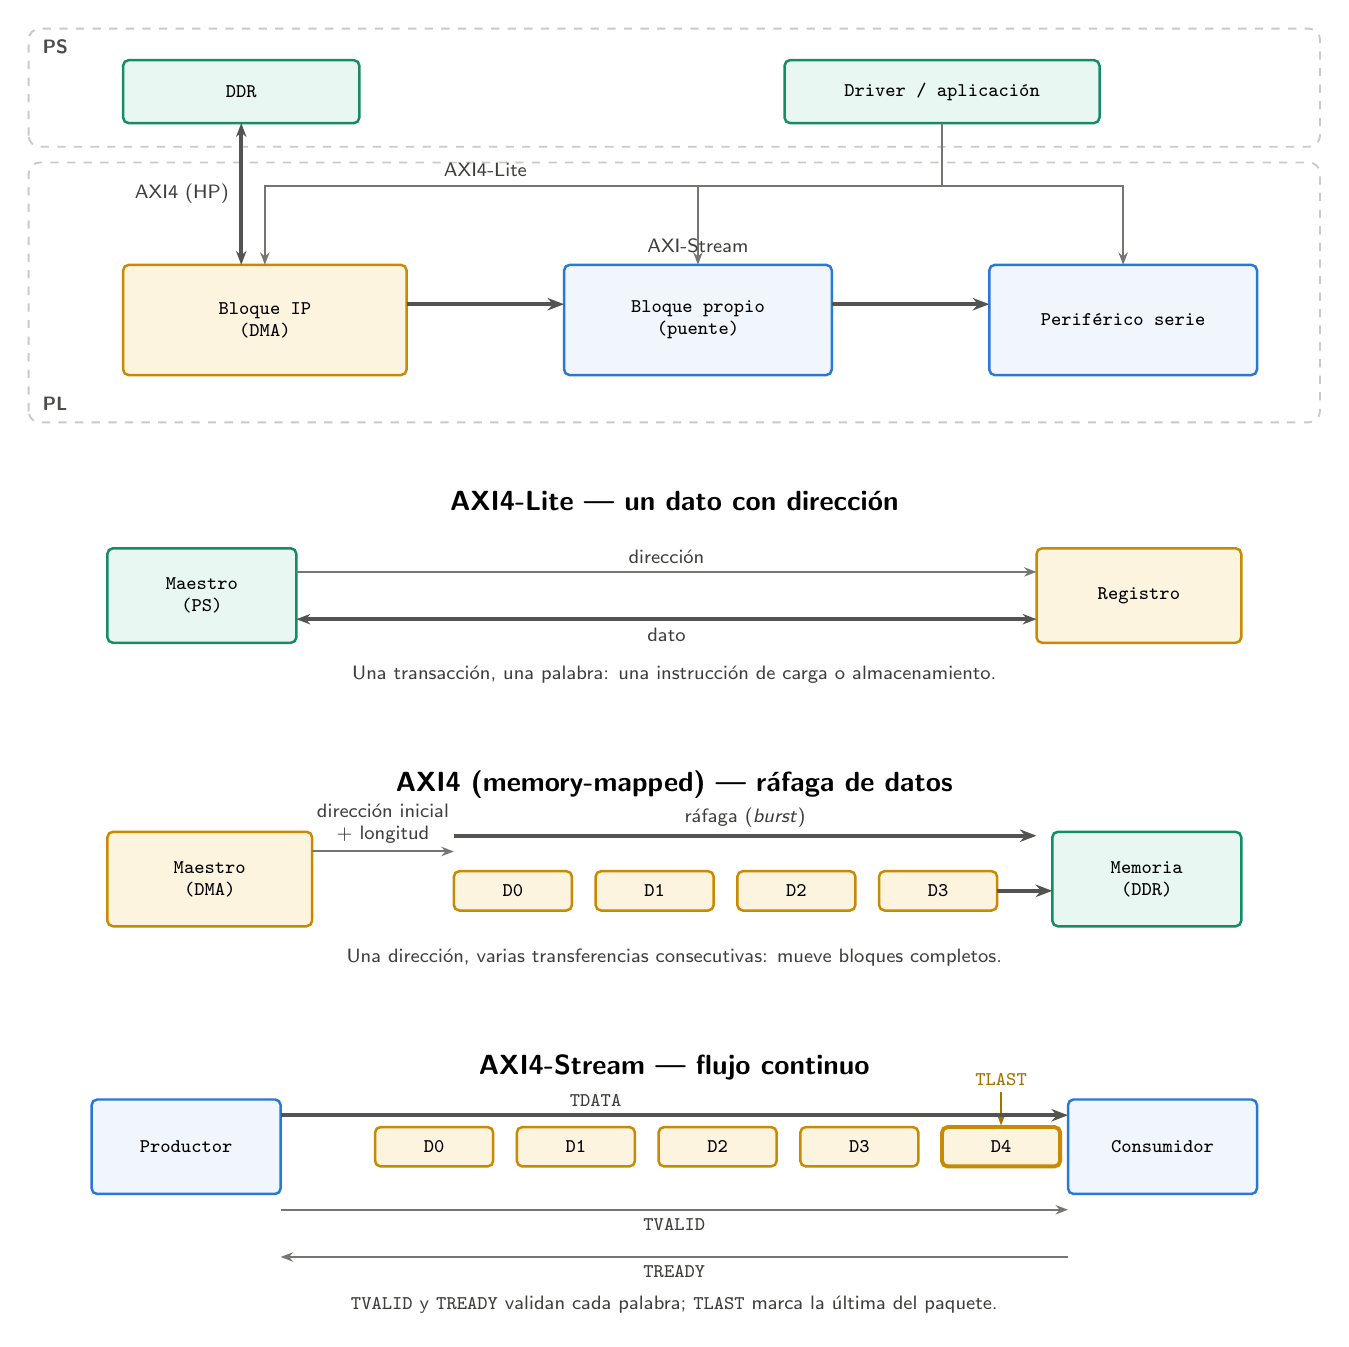
\begin{tikzpicture}[
    x=1cm, y=1cm, font=\sffamily\small,
    blk/.style={draw=cPropio, line width=0.9pt, rounded corners=2pt,
                fill=cPropio!7},
    ip/.style={draw=cIP!85!black, line width=0.9pt, rounded corners=2pt,
               fill=cIP!12},
    ext/.style={draw=cExt!80!black, line width=0.9pt, rounded corners=2pt,
                fill=cExt!10},
    band/.style={draw=cRef!45, dashed, line width=0.7pt, rounded corners=4pt},
    sig/.style={-{Stealth[length=4.5pt]}, line width=0.7pt, cRef!85!black},
    stream/.style={-{Stealth[length=6pt]}, line width=1.5pt, cRef!60!black},
    lbl/.style={font=\sffamily\scriptsize, inner sep=2pt},
    tlbl/.style={font=\ttfamily\scriptsize, inner sep=2pt},
    name/.style={font=\ttfamily\scriptsize, align=center},
]

% ===========================================================================
% Vista de conjunto: qué perfil circula por dónde
% ===========================================================================
\draw[band] (-0.2,16.05) rectangle (16.2,17.55);
\node[lbl, anchor=north west, text=cRef!55!black] at (-0.1,17.48) {\textbf{PS}};

\draw[band] (-0.2,12.55) rectangle (16.2,15.85);
\node[lbl, anchor=south west, text=cRef!55!black] at (-0.1,12.62) {\textbf{PL}};

% ----- PS -----
\draw[ext] (1.0,16.35) rectangle (4.0,17.15);
\node[name] at (2.5,16.75) {DDR};

\draw[ext] (9.4,16.35) rectangle (13.4,17.15);
\node[name] at (11.4,16.75) {Driver / aplicación};

% ----- PL -----
\draw[ip] (1.0,13.15) rectangle (4.6,14.55);
\node[name, align=center] at (2.8,13.85) {Bloque IP\\(DMA)};

\draw[blk] (6.6,13.15) rectangle (10.0,14.55);
\node[name, align=center] at (8.3,13.85) {Bloque propio\\(puente)};

\draw[blk] (12.0,13.15) rectangle (15.4,14.55);
\node[name] at (13.7,13.85) {Periférico serie};

% ----- AXI4-Lite: configuración desde el driver -----
\draw[sig] (11.4,16.35) -- (11.4,15.55) -- (2.8,15.55) -- (2.8,14.55);
\draw[sig] (11.4,15.55) -- (8.3,15.55) -- (8.3,14.55);
\draw[sig] (11.4,15.55) -- (13.7,15.55) -- (13.7,14.55);
\node[lbl, anchor=south, text=cRef!45!black] at (5.6,15.60) {AXI4-Lite};

% ----- AXI4 hacia la DDR por el puerto de alto rendimiento -----
\draw[{Stealth[length=5pt]}-{Stealth[length=5pt]}, line width=1.5pt, cRef!60!black]
      (2.5,16.35) -- (2.5,14.55);
\node[lbl, anchor=east, text=cRef!45!black] at (2.42,15.45) {AXI4 (HP)};

% ----- AXI-Stream entre bloques de la PL -----
\draw[stream] (4.6,14.05) -- (6.6,14.05);
\draw[stream] (10.0,14.05) -- (12.0,14.05);
\node[lbl, anchor=south, text=cRef!45!black] at (8.3,14.63) {AXI-Stream};

% ===========================================================================
% (a) AXI4-Lite -- un dato con dirección
% ===========================================================================
\node[lbl, font=\sffamily\bfseries\normalsize] at (8.0,11.55)
      {AXI4-Lite --- un dato con dirección};

\draw[ext] (0.8,9.75) rectangle (3.2,10.95);
\node[name] at (2.0,10.35) {Maestro\\(PS)};

\draw[ip] (12.6,9.75) rectangle (15.2,10.95);
\node[name] at (13.9,10.35) {Registro};

\draw[sig] (3.2,10.65) -- (12.6,10.65);
\node[lbl, anchor=south, text=cRef!45!black] at (7.9,10.68) {dirección};

\draw[{Stealth[length=5pt]}-{Stealth[length=5pt]}, line width=1.3pt, cRef!60!black]
      (3.2,10.05) -- (12.6,10.05);
\node[lbl, anchor=north, text=cRef!45!black] at (7.9,10.02) {dato};

\node[lbl, text=cRef!45!black, align=center] at (8.0,9.35)
      {Una transacción, una palabra: una instrucción de carga o almacenamiento.};

% ===========================================================================
% (b) AXI4 memory-mapped -- ráfaga
% ===========================================================================
\node[lbl, font=\sffamily\bfseries\normalsize] at (8.0,7.95)
      {AXI4 (\textit{memory-mapped}) --- ráfaga de datos};

\draw[ip] (0.8,6.15) rectangle (3.4,7.35);
\node[name] at (2.1,6.75) {Maestro\\(DMA)};

\draw[ext] (12.8,6.15) rectangle (15.2,7.35);
\node[name] at (14.0,6.75) {Memoria\\(DDR)};

\draw[sig] (3.4,7.10) -- (5.2,7.10);
\node[lbl, anchor=south, text=cRef!45!black, align=center] at (4.3,7.13)
      {dirección inicial\\+ longitud};

\foreach \x/\d in {5.2/D0, 7.0/D1, 8.8/D2, 10.6/D3} {
    \draw[ip] (\x,6.35) rectangle (\x+1.5,6.85);
    \node[tlbl] at (\x+0.75,6.60) {\d};
}
\draw[stream] (5.2,7.30) -- (12.6,7.30);
\node[lbl, anchor=south, text=cRef!45!black] at (8.9,7.33) {ráfaga (\textit{burst})};
\draw[stream] (12.1,6.60) -- (12.8,6.60);

\node[lbl, text=cRef!45!black, align=center] at (8.0,5.75)
      {Una dirección, varias transferencias consecutivas: mueve bloques completos.};

% ===========================================================================
% (c) AXI4-Stream -- flujo continuo con handshake
% ===========================================================================
\node[lbl, font=\sffamily\bfseries\normalsize] at (8.0,4.35)
      {AXI4-Stream --- flujo continuo};

\draw[blk] (0.6,2.75) rectangle (3.0,3.95);
\node[name] at (1.8,3.35) {Productor};

\draw[blk] (13.0,2.75) rectangle (15.4,3.95);
\node[name] at (14.2,3.35) {Consumidor};

\foreach \x/\d in {4.2/D0, 6.0/D1, 7.8/D2, 9.6/D3} {
    \draw[ip] (\x,3.10) rectangle (\x+1.5,3.60);
    \node[tlbl] at (\x+0.75,3.35) {\d};
}
\draw[ip, line width=1.4pt, draw=cIP!85!black] (11.4,3.10) rectangle (12.9,3.60);
\node[tlbl] at (12.15,3.35) {D4};
\draw[sig, cIP!70!black] (12.15,4.05) -- (12.15,3.62);
\node[lbl, anchor=south, text=cIP!70!black] at (12.15,4.05) {\texttt{TLAST}};

\draw[stream] (3.0,3.75) -- (13.0,3.75);
\node[tlbl, anchor=south, text=cRef!45!black] at (7.0,3.78) {TDATA};

\draw[sig] (3.0,2.55) -- (13.0,2.55);
\node[tlbl, anchor=north, text=cRef!45!black] at (8.0,2.52) {TVALID};

\draw[sig] (13.0,1.95) -- (3.0,1.95);
\node[tlbl, anchor=north, text=cRef!45!black] at (8.0,1.92) {TREADY};

\node[lbl, text=cRef!45!black, align=center] at (8.0,1.35)
      {\texttt{TVALID} y \texttt{TREADY} validan cada palabra; \texttt{TLAST} marca la última del paquete.};

\end{tikzpicture}
\end{document}
